\chapter{Graph Traversal}

Permasalahan paling mendasar dari sebuah graph adalah mengunjungi setiap edge dan vertex dari sebuah graph dalam cara yang sistematik. Untuk menyelesaikan permasalahan tersebut maka kita memerlukan sebuah algoritma graph traversal. Ide dasar dari sebuah graph traversal adalah menandai (marking) setiap vertex yang telah kita kunjungi dan menjelajahi vertex yang belum kita kunjungi.

Pada umumnya, kita beri 3 tanda pada setiap vertex sebagai berikut.
\begin{enumerate}
	\item Belum dikunjungi (\textit{undiscovered}), vertex yang masih dalam kondisi awal. Umumnya ditandai dengan warna putih.
	\item Sudah dikunjungi (\textit{discovered}), vertex yang sudah dikunjungi tetapi masih belum menjelajahi tetangga dari vertex tersebut. Umumnya ditandai dengan warna abu-abu.
	\item Sudah diproses (\textit{processed}), vertex yang sudah dikunjungi dan semua tetangga juga sudah dijelajahi. Umumnya ditandai dengan warna hitam.
\end{enumerate}

Sebuah vertex berubah tanda secara bertahap dari \textit{Undiscovered} menjadi \textit{Discovered} dan terakhir menjadi \textit{Processed}. 

Ada 2 algoritma Graph Traversal yang populer yaitu \textit{Breadth-First Search} dan \textit{Depth-First Search}. Masih ada banyak metode Graph Traversal yang lain tetapi itu tidak dibahas di materi ini. Mahasiswa diharapkan untuk mencari tau jenis-jenis Graph Traversal yang lain.

\section{Breadth-First Search}

\textit{Breadth-First Search} (BFS) merupakan metode Graph Traversal yang paling sederhana dan menjadi dasar dari banyak algoritma graph lainnya seperti algoritma Djikstra untuk mencari jalur terpendek dan algoritma Prim untuk mencari minimum spanning tree.

Diberikan sebuah graph $G = (V,E)$ dan sebuah vertex awal $s$, maka algoritma \textit{Breadth-First Search} akan menjelajahi setiap edge dari G untuk menemukan semua vertex yang bisa dicapai dari $s$. \textit{Breadth-First Search} juga dapat mencari jumlah edge minimal (tanpa menghitung bobot edge) untuk mencapai sebuah vertex tertentu. Algoritma BFS bisa digunakan di graph berarah atau tidak berarah. Kompleksitas waktu dari BFS adalah O(V+E).

Illustrasi BFS bisa dilihat di ~\ref{fig:BFS}.

\begin{figure}
    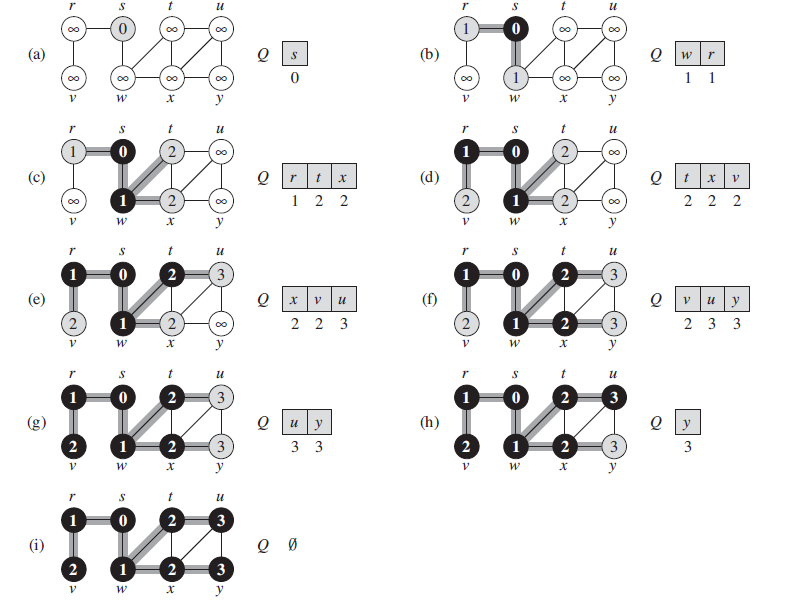
\includegraphics[width=\textwidth,keepaspectratio]{fig/BFS.png}%
	\caption{Illustrasi BFS}%
	\label{fig:BFS}%
\end{figure}

\subsection{Implementasi Breadth-First Search}

Implementasi lengkap dari BFS bisa dilihat dari Algoritma~\ref{algo:migraph-BFS}.

\lstinputlisting[language=Python, 
                 firstline=116,
                 lastline=143,
                 label={algo:migraph-BFS},
                 caption=Implementasi BFS
                ]
                {code/migraph.py}

Fungsi BFS akan menerima satu parameter yaitu vertex sumber $s$ dimana kita akan mulai menjelajahi.

\lstinputlisting[language=Python, 
                 firstline=116,
                 lastline=116,
                 label={algo:migraph-BFS-def},
                 caption=Definisi fungsi BFS
                ]
                {code/migraph.py}

Sebelum memasuki inti dari algoritma BFS, pertama kita deklarasi beberapa variabel untuk BFS yang bisa dilihat di Algo ~\ref{algo:migraph-variabel-BFS}. Variabel $i$, digunakan ketika kita akan mencetak langkah traversal dari BFS. Dengan variabel $i$ kita bisa mengetahui vertex mana yang dikunjungi terlebih dahulu dan selanjutnya. Variabel $traversal$ untuk menyimpan semua urutan kunjungan vertex. Kedua variabel $i$ dan $traversal$ hanya untuk keperluan cetak dan bukan bagian dari BFS. 

Variabel $\_\_color$ digunakan untuk mewarnai setiap vertex yang dikunjungi. Ada tiga warna yaitu $WHITE$, $GRAY$ dan $BLACK$. Variabel $\_\_distance$ untuk mengetahui jarak dari sebuah vertex dari source (vertex awal). Variabel $\_\_predecessor$ untuk mengetahui \textit{predecessor} (parent) dari sebuah vertex. 

\lstinputlisting[language=Python, 
                 firstline=117,
                 lastline=120,
                 label={algo:migraph-variabel-BFS},
                 caption=Variabel BFS
                ]
                {code/migraph.py}

Setelah kita deklarasi, kita definisikan variabel $\_\_color$ dan $\_\_distance$. Semua vertex awalnya berwarna putih dan jaraknya INF. $\_\_predecessor$ tidak usah didefinisikan karena memang nilai awalnya adalah NONE.

\lstinputlisting[language=Python, 
                 firstline=121,
                 lastline=123,
                 label={algo:migraph-define-variabel-BFS},
                 caption=Definisi Variabel BFS
                ]
                {code/migraph.py}

Kita definisikan warna dari vertex $s$ sebagai warna $GRAY$ menandakan vertex sudah dikunjungi tetapi belum semua tetangga dikunjungi dan jarak bernilai 0.

\lstinputlisting[language=Python, 
                 firstline=124,
                 lastline=125,
                 label={algo:migraph-define-s-BFS},
                 caption=Definisi Variabel S BFS
                ]
                {code/migraph.py}

Untuk melacak vertex mana yang sudah dikunjungi kita akan gunakan \textit{Queue} $Q$. Di python, untuk menyederhanakan kita bisa menggunakan \textit{list} yang bisa dilihat di Algo ~\ref{algo:migraph-queue-BFS}. Kita masukkan dulu vertex $s$ ke dalam \textit{Queue} menandakan kita sedang mengunjungi vertex $s$.

\lstinputlisting[language=Python, 
                 firstline=126,
                 lastline=127,
                 label={algo:migraph-queue-BFS},
                 caption=Penggunaan Queue BFS
                ]
                {code/migraph.py}

$Q$ berfungsi sebagai penanda kunjungan kita ke setiap vertex. Semua vertex yang akan kita kunjungi akan kita masukkan dari belakang (\textit{append}) variabel $Q$. Semua tetangga dari vertex $s$ akan kita \textit{append} ke dalam $Q$. Setelah itu kita akan proses dari depan satu persatu. Setiap kita proses satu vertex, kita \textit{append} semua tetangga dari vertex tersebut untuk dikunjungi nanti.

Kita akan looping terus menerus dan lakukan proses di atas sampai semua vertex sudah dikunjungi atau $Q$ tidak berisi lagi (lihat ~\ref{algo:migraph-queue-while-BFS}).

\lstinputlisting[language=Python, 
                 firstline=129,
                 lastline=129,
                 label={algo:migraph-queue-while-BFS},
                 caption=Looping selama masih ada isi di Queue.
                ]
                {code/migraph.py}
								
Di awal dari looping, kita akan mengeluarkan vertex paling depan dari $Q$ untuk diproses. 

\lstinputlisting[language=Python, 
                 firstline=130,
                 lastline=130,
                 label={algo:migraph-queue-pop-BFS},
                 caption=Keluarkan isi vertex yang berada di tempat terdepan Queue.
                ]
                {code/migraph.py}

Kita akan memproses vertex yang dikeluarkan ($u$) jika warna dari vertex $u$ adalah $WHITE$ (artinya belum pernah dikunjungi sebelumnya). Pertama kita akan melihat semua tetangga dari vertex $u$. Setiap tetangga tersebut ($v$) kita akan beri warna $GRAY$ menandakan sudah dikunjungi tetapi belum mengunjungi tetangganya. Kemudian kita tambah jarak vertex tersebut 1 (jarak menandakan jarak dari $s$ ke vertex tersebut). Kemudian kita set \textit{predecessor} dari semua vertex tetangga menjadi $u$. Yang terakhir semua tetangga dimasukkan ke belakang dari $Q$.

\lstinputlisting[language=Python, 
                 firstline=136,
                 lastline=141,
                 label={algo:migraph-queue-process-BFS},
                 caption=Proses vertex yang dikeluarkan dari Queue.
                ]
                {code/migraph.py}

Setelah diproses, vertex $u$ tersebut diberi warna $BLACK$ yang artinya sudah dikunjungi dan semua tetangga juga sudah dikunjungi.

\lstinputlisting[language=Python, 
                 firstline=142,
                 lastline=142,
                 label={algo:migraph-vertex-Black-BFS},
                 caption=Vertex diberi warna hitam.
                ]
                {code/migraph.py}
								
Setiap kali kita memproses sebuah vertex, kita akan simpan ke dalam variabel $traversal$ untuk mencatat kunjungan kita. Baris ini bukan bagian dari BFS tetapi hanya untuk keperluan mencatat saja.

\lstinputlisting[language=Python, 
                 firstline=131,
                 lastline=134,
                 label={algo:migraph-traversal-BFS},
                 caption=Mencatat kunjungan dalam traversal.
                ]
                {code/migraph.py}
								
\section{Depth-First Search}

Strategi dari \textit{Depth-First Search} (DFS) berbeda dari BFS dimana BFS mengunjungi terlebih dahulu semua tetangga, maka DFS mengunjungi satu vertex secara mendalam sampai tidak bisa dikunjungi lagi baru pindah ke tetangga baru. Kompleksitas waktu dari DFS sama seperti BFS, O(V+E), akan tetapi untuk graph yang sangat besar sekali DFS bisa terlalu dalam menjelajahi satu verteks tanpa menjelajahi verteks lain.

Illustrasi DFS bisa dilihat di ~\ref{fig:Dfs}.

\begin{figure}
    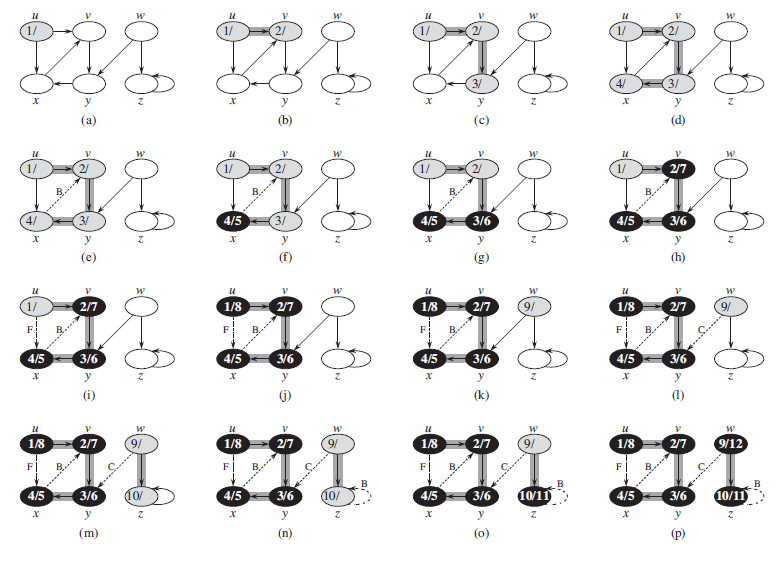
\includegraphics[width=\textwidth,keepaspectratio]{fig/DFS.png}%
	\caption{Illustrasi DFS}%
	\label{fig:Dfs}%
\end{figure}


\subsection{Implementasi Depth-First Search}

Implementasi lengkap dari BFS bisa dilihat dari Algo~\ref{algo:migraph-DFS}. Algoritma dari DFS merupakan algoritma rekursif.

\lstinputlisting[language=Python, 
                 firstline=88,
                 lastline=115,
                 label={algo:migraph-DFS},
                 caption=Implementasi DFS
                ]
                {code/migraph.py}

Pada fungsi $DFS\_traversal(s)$, semua verteks akan diwarnai dengan warna $WHITE$ terlebih dahulu. Setelah itu kita akan mulai mengunjungi dari vertex $s$. Kunjungan akan ditandai dengan memanggil fungsi $DFS\_visit$

\lstinputlisting[language=Python, 
                 firstline=88,
                 lastline=98,
                 label={algo:migraph-DFS-2},
                 caption=Implementasi DFS
                ]
                {code/migraph.py}

Fungsi $DFS\_visit$ akan mengunjungi semua vertex beserta anaknya sampai yang paling dalam. Inti dari DFS adalah pada rekursif, dimana setiap tetangga vertex $v$ yang berwarna $WHITE$ akan dikunjungi dan ketika rekursif selesai, vertex $v$ tersebut akan diwarnai $BLACK$.

\lstinputlisting[language=Python, 
                 firstline=99,
                 lastline=114,
                 label={algo:migraph-DFS-3},
                 caption=Implementasi DFS
                ]
                {code/migraph.py}

